
\subsection{Pictures used}
\subsubsection{adada}


\noindent
Cover picture filename (in titlepage): \texttt{cover}\\
Logo filename (in foot): \texttt{logo}

\subsection{Boxes}

\begin{verbatim}
\fullboxbegin
Content
\fullboxend
\end{verbatim}

\begin{verbatim}
\leftboxbegin
Content
\leftboxend
\end{verbatim}

\begin{verbatim}
\rightboxbegin
Content
\rightboxend
\end{verbatim}

\begin{verbatim}
\frameboxbegin{Frame Title}
Content
\frameboxend
\end{verbatim}

\newpage

\section{First section}
\lipsum[1]

\fullboxbegin
\lipsum[1]
\fullboxend

\lipsum[1]

\subsection{First subsection}
\lipsum[1]
\subsubsection{asas}
\subsubsection*{asas}


\lipsum[1-2]

\rightboxbegin
\begin{itemize}
 \item Lorem ipsum
 \item Lorem ipsum
\end{itemize}
\rightboxend

\lipsum[1]

\subsubsection{First subsubsection}

\lipsum[1]

\begin{figure}[!h]
\centering

\includegraphics[width=0.5\textwidth]{sky.jpg}
\caption{The sky is the limit.}
\end{figure}

\section*{Unnumbered section}
\lipsum[1]

\begin{figure}[!h]
\centering

\includegraphics[width=0.5\textwidth]{sky.jpg}
\caption*{The sky is the limit.}
\end{figure}

\section{Second section}

\lipsum[1]
\begin{table}[!h]
\centering
\caption{Sample table.}
\begin{tabular}{cccc}
\toprule
Value 1 & Value 2 & Value 3 & Value 4\\
\midrule
 odd     & odd   & odd & 1.00 \\
 even    & even  & even& 1.00 \\
 odd     & odd   & odd & 1.00 \\
 even    & even  & even& 1.00 \\
\bottomrule
\end{tabular}
\end{table}

\lipsum[1]

\frameboxbegin{Sample frame}
\lipsum[1]
\frameboxend


\section{ccOS 모듈 View}
ccOS의 모듈은 메니저와 엔진으로 이루어 진다. 이번 섹션은 ccOS의 모듈을 이루는 메니저와 엔진을 설명한다. 
\subsection{ccOS 메니저}
ccOS에서 Manager들의 역할은 ccOS Application들 간의 상호 동작시 필요한 각종 Policy(사양)을 관리/적용하기 위해 도입된 System Application들로서,ccOS는 이 Manager들을 통해 Application들 간에 화면 천이 사양,멀티미디어 자원할당 등을 관리하며, Application 기동 및 동작 중 Lifecycle 관리 및 예외 사항 발생에 대한 처리를 담당한다.
현재까지 개발된 Manager에 대한 설명은 다음과 같으며, 추후 필요에 의해 추가될 수 있다.

\subsubsection{AppManager}
%\subsection{AppManager}
ccOS Application들의 Lifecycle을 관리하는 system application으로서 Application lifecycle 에 따라 등록된 lifecycle callback을 호출하며 필요시 다른 system applicaion들에게 등 록된 Application정보를 전달한다.

\subsubsection{AppEventMgr}
System Key (Hard Key 중 ) or Application을 변경하는 Softkey를 받아, 해당하는 Application에게 전달하는 역할을 하며, 화면 구성 및 변경에 대한 Policy를 적용하는 역할을 하 는 System Application
\subsubsection{IACManager}
Application 및 Manager들간의 IPC를 위한 Abstract communicator 이며, 기존 IPC와 같은 low level 형태의 통신 함수 및 service Type, App type을 이용한 수신자를 명확하게 지 정하지 않고 intent 기반의 통신 방법도 제공한다.

\subsection{ccOS Engines}
\subsubsection{Audio Engine}
\subsubsection*{개요} Audio는 audio의 설정, PCM stream in/out, focus관리 등의 ccOS audio 전반의 기능을 담당하는 interface이다. Audio는 audio의 설정, PCM stream in/out, focus관리 등의 ccOS audio 전반의 기능을 담당하는 interface이다. Audio는 audio의 설정, PCM stream in/out, focus관리 등의 ccOS audio 전반의 기능을 담당하는 interface이다.
\begin{itemize}
	\item Audio는 audio의 설정, PCM stream in/out, focus관리 등의 ccOS audio 전반의 기능을 담당하는 interface이다.
	\item Audio모듈은 HAudio와 HAudioFocus interface를 제공한다.
	\item Audio의 구현은 HAudioEngine과 HAudioFocusEngine에 정의되어 있으며 HAudio와 HAudioFocus interface를 통해 구현부에 접근할 수 있다. 단, HAudio의 stream API의 경우 pulse audio나 alsa에 직접 접근한다.
	\item System application으로서 AudioFocusMgr를 제공한다. AudioFocusMgr은 HAudio의 interface set을 이용하여 application에 user friendly한 convenient api를 제공한다
\end{itemize}

\subsubsection*{Audio Interface}
Audio Interface는 HAudio, HAudioFocus로 구성된다. 
	\paragraph{HAudio} Audio source와 sync의 pair인 stream의 설정을 및 audio data를 관리한다.

	HAudio의 interface는 HAudioConfig와 HAudioControl 로 구체화 된다.

	\subparagraph{HAudioConfig}
	ccOS audio의 설정 기능을 담당한다.
	\begin{enumerate}
		\item Equalizer와 preset
		\item 믹싱 우선순위
		\item Speed dependent 볼륨 설정
		\item 터치음 enable / disable 설정
	\end{enumerate}


	\subparagraph{HAudioControl}
	Source와 sync를 관리한다.
	\begin{enumerate}
		\item Audio source와 sync 연결 및 연결해지
		\item 연결된 audio source 목록 관리
		\item 각기 source/sync의 볼륨 조절
		\item 마이크 게인 조절
\end{enumerate}

\subsubsection{Layout}
\begin{figure}[h]
\centering
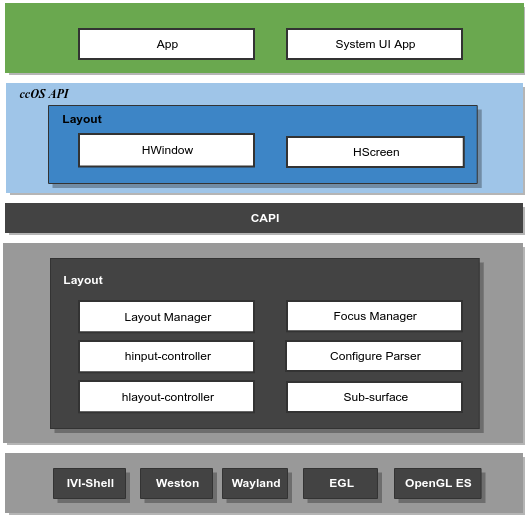
\includegraphics[width=1\textwidth]{fig/layout_engine.png}
\caption{Layout Engine 구조}
\end{figure}
Layout은 ccOS HLayout API, HLayout Engine, Wayland로 구성 되고 이들 간 통신을 통해 윈도우를 생성/소멸 및 레이아웃을 관리 한다.

 API는 HScreen과 HWindow를 통해 레이아웃을 조절을 위한 인터페이스를 제공한다.

    HScreen
        화면 개수 및 사용 유무를 확인 하고 화면의 배경을 설정 할 수 있다. 화면은 사용자의 입력을 받을 수 있는 윈도우 포커스를 갖는데 각 화면 당 1개가 할당 되며 이는 HScreen을 통해 직접 또는 입력 키에 따라 포커스를 설정 할 수 있다.
        화면에 표시 될 여러 윈도우의 위치를 지정 할 수 있으며 이를 통해 레이어 별 레이아웃을 조절 할 수 있다.
    HWindow
        각 어플리케이션의 윈도우 위치를 조절하거나 visibility를 설정 할 수 있으며 이벤트를 받아 어플리케이션에 알리는 역할을 수행 한다. 관련 이벤트는 포커스, 키\&노브 입력, 언어 변경, layout 변경에 따른 윈도우 표시 유무를 나타내는 이벤트 등이 있다.

Engine은 API를 통해 전달 된 사용자 입력을 처리하고 이를 Wayland에 전달하는 역할을 수행하며 Layout(Geometry), Focus를 관리한다.

    Layout 관리
        화면을 구성하는 레이어, 서페이스, 순서 등을 관리하며 위치 및 fade를 조절하여 transition 처리를 수행한다. Geometry 구성 및 transition 처리는 스크립트를 통해 수행 되고 사용자 입력에 의해 스크립트 동작을 수행 한다.
    Focus 관리
        윈도우 간 포커스를 관리하며 윈도우의 show/hide에 따라 포커스 자동 이동도 수행한다. 단지 윈도우 간 포커스를 관리 할 뿐 윈도우 내부 구성 요소 간 포커스에 대해서는 관여하지 않는다.
    hlayout-controller
        ivi-layout을 호출하여 geometry 설정 정보를 전달하는 프로토콜 구현부이다. 이 controller를 통해 IVI-shell과 통신을 한다.
    hinput-controller
        ivi-shell의 input 모듈로 wayland에서 전달 되는 모든 input 정보를 조절한다.
    Configure Parser
        Layout을 json 형식으로 작성하고 engine이 동작하는 동안 layout을 동적으로 적용 할 수 있도록 한다.
    Sub-surface
        main surface에 종속 된 surface 생성이 필요한 경우 생성,소명, 관리하는 역할을 수행한다.

Wayland는 Engine에서 구성한 geometry에서 대해 IVI-shell에 기반하여 플러그인을 통해 조절한다.

    IVI-Shell
        IVI용 shell 프로토콜로써 engine에서 제공하는 플러그인을 로딩하고 weston 및 wayland와 통신할 수 있도록 한다.
    Weston
        Wayland 컴포지터로 윈도우를 구성하는 surface에 대한 그래픽 조합 작업을 수행한다.
    Wayland
        Display 서버 역할을 수행한다. 클라이언트 프로토콜을 제공하여 윈도우에 대한 관리, 컴포지팅을 할 수 있도록 한다.



\subsubsection{Media 엔진}
\subsubsection*{개요}
%\begin{figure}[!h]
\begin{figure}[h]
\centering
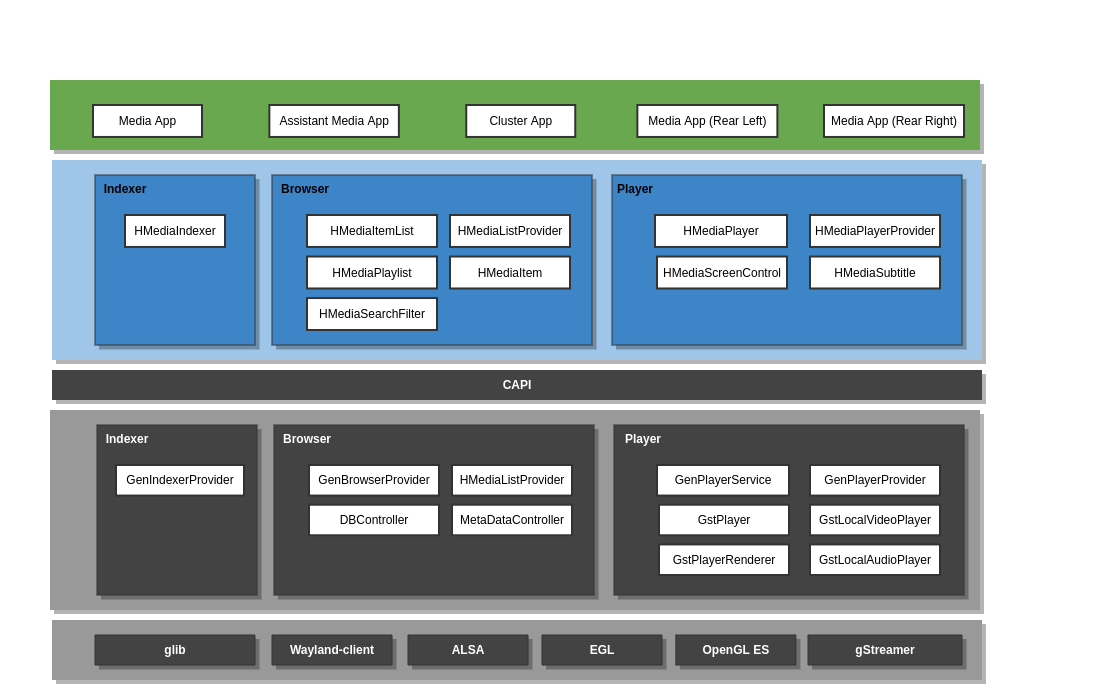
\includegraphics[width=0.8\textwidth]{fig/media_engine.png}
\caption{Media Engine architecture}
\end{figure}
위에 보는 그림은 Media와 관련된 S/W 구성 요소들만 표현한 Layered diagram 입니다. 최 상단에 Media application과 Assistant Media application, Cluster application, 그리고 후석 좌/우 좌석 에서 동작하는 Media App들이 표현 되어 있습니다.

각 미디어 앱들은 ccOS API layer에 위치하고 있는 API들을 사용하여 미디어 재생, 미디어 meta data 검색과 같은 기능을 수행할 수 있습니다. ccOS layer에 위치하고 있는 Media app은 크게 3 가지 category로 구분됩니다. 각각 Indexer, Browser, Player 입니다.
\subsubsection*{Media API}
Media엔진 API는 3개의 기능을 지원하기 위하여 각 기능별로 API를 분류 하였다.
\paragraph{Indexer} 
\subparagraph{HMediaIndexer}
Indexer API에는 HMediaIndexer class가 있습니다. 이 class는 Head unit에 연결된 media storage (ex. USB thumb drive 등) 내에 존재하는 여러 미디어 content들을 scan 한 후 각 content들에 대한 이름, 파일위치, 코덱 정보, thumbnail image등의 meta data들을 특정 위치에 caching 하는 기능을 수행 합니다. 이후 application layer에서는 Browser에서 제공하 는 API를 통해 Indexer를 통해 추출된 미디어 meta data에 접근할 수 있습니다.

ii. HMediaIndexer는 indexing의 start, stop과 indexing 상태를 원하는 시점에서 query 하는 getIndexingStatus, 그리고 indexing 상태의 변화를 비동기로 전달 받기 위해 listener를 설 정하는 setEventListener 함수를 제공합니다.

\paragraph{Browser}
Browser category 내의 API들은 Indexer를 통해 생성된 다양한 meta data를 접근하는 기능을 제공합니다. Browser API 내 각각의 class들에 대한 설명은 다음과 같습니다.
\subparagraph{HMediaListProvider}
HMediaItemList와 HMediaPlaylist를 생성하고 내용을 채워 넣는 기능을 제공합니다. 뿐만아니라 이미 생성되어 있는 HMediaItemList/HMediaPlaylist를 획득하는
기능을 제공합니다. 이미 생성된 MediaItemList의 획득 기능은 “전석/후석 완전 독립 시스템”이라는 신규 사양 중 동시에 2개의 미디어 앱이 서로 다른 좌석의 화면
에서 독립적으로 실행되나 동일한 재생화면 혹은 동일한 list 화면을 보여 주는데 필요한 기능입니다.
\subparagraph{HMediaItemList}
HMediaItem들을 관리하는 기능을 제공합니다. HMediaItem을 추가한다던가 제거할 수 있으며, 특정 index에 위치하는 HMediaItem을 획득하는데 사용될 수 있습 니다. save 함수를 호출할 경우 해당 lits가 engine 내 저장되어 있지 않을 시 해당 list를 engine 내 저장합니다. 이미 저장된 list의 경우 sync 기능 호출 시, API layer와 engine layer 간 차이점을 동기화 합니다.
\subparagraph{HMediaPlayrlist}
HMediaItemList와 유사하나 Play list는 application에서 마음대로 수정 가능한 list로 처리 됩니다.
\subparagraph{HMediaItem}
각각의 media item에 대해 여러 meta data를 제공하기 위해 존재하는 class 입니다. Meta data를 실제로 유지하는 class는 HMetaItemDataType class이며 HMediaItem
하나의 instance는 HMetaItemDataType instance 하나를 보유합니다.
\subparagraph{HMediaSearchFilter}
MediaList 생성 후 MediaList 내에 item을 채우고자 할 때 HMediaListProvider의 fillMediaItems를 호출합니다. 이 때 HMediaListFillParamType 객체를 argument로 넣어 줍니다. HMediaListFillParamType는 어떤 data를 채워 넣을지 filtering 하는 다양한 조건들을 지정하는데 사용됩니다. 이 중 HMediaSearchFilter 객체를 지정해 줄 수 있는데, 이 객체를 통해 특정 title 명, artist 이름, album 명에 해당하는 item만 검색 하여 list를 채울 수 있습니다.

\paragraph{Player}
\subparagraph{HMediaPlayer}
Playback 시 사용하는 class 입니다. Player 객체는 local audio player, local video player, streaming audio player, streaming video player 등으로 생성될 수 있습니다. 생성 후 설정된 URL을 통해 gStreamer media pipeline을 형성한 후 media content를 재생하는 기능을 제공합니다.
\subparagraph{HMediaPlayerProvider}
MediaPlayer를 생성 혹은 이미 생성된 player의 handle을 획득하는데 사용되는 class 입니다. Player의 생성 시 unique한 이름을 줘서 생성한 후 다른 application과 player를 공유할 수 있습니다. 혹은 anonymous player를 생성하여 하나의 application process 내에서만 생성하여 사용할 수도 있습니다.
\subparagraph{HMediaSubtitle}
HMediaScreenControl과 마찬가지로 영상을 화면상에 출력할 필요가 있는 player의 경우, 자막까지 출력할 필요가 있을 시 사용되는 class 입니다. HMediaSubtitle class는
자막의 활성화 및 비활성화, 자막 크기의 설정등을 수행하는데 사용될 수 있습니다.

\subsubsection{Recorder}
\subsubsection*{개요}
그림에서 voice recorder app은 사용자의 음성을 녹음하여 file로 저장하는 기능을 수행하는 application 입니다. 앱은 HRecorder API를 사용해 voice recording 작업을 수행합니다. Recorder engine 내부에는 API layer와 마찬가지로 AudioRecorder가 존재하며 audio recording 작업을 수행합니다. 실질적인 Audio recording은 media playback의 경우와 마찬가지로 gStreamer media
pipeline을 사용하며, 이 때 해당 pipeline의 front-end 입력은 mic이며 back-end sink는 file 입니다. 다음은 API에 대한 설명입니다.

\subsubsection*{Recorder API}
\paragraph{HAudioRecorder}
Recording을 수행하고 싶은 application에서 audio recording을 제어하고 싶을 때 사용해야 하는 기능들을 제공하는 class 입니다. HAudioRecorder class는 여러 개의 객체로 인스턴스화 될 수 있으며 각 객체의 인스턴스화 때 생성자를 통해 혹은 여러 setting과 관련된 member function들을 통해 상세한 녹음의 설정이 가능합니다. 주요 설정 사항은 다음과 같습니다.
\begin{itemize}
	\item RecordCodecType : Recording 된 음성 data를 file로 저장할 때 어떠한 압축 코덱을 사용할지 지정할때 사용됩니다. 압축 codec type에는 MP3, AMR, AAC, RAW 등이 지정될 수 있습니다.
	\item RedordContainerType : file에 data를 저장하는 형태를 규정하는 file container type을 지정할때 사용되는 type 입니다. WAV, PCM, MP3등이 지정될 수 있습니다.
	\item AudioRecordSource : 저장할 sound data의 source를 지정하는 type 입니다. 기본적으로 mic를 지원하며, 필요 시 voice call, connectivity phone등이 추가될 수 있습니다.
\end{itemize}
\paragraph{HAudioRecordItem}
각각의 저장된 item은 AudioRecordItem을 통해 관리됩니다. 저장된 item에 대해 duration, date, title등의 data를 유지하며, application에서 이와같은 data를 query 하는데 사용될 수 있는
기능들을 제공합니다.
\paragraph{IHAudioRecorderListener}
IHAudioRecorderListener는 HAudioRecorder 객체 생성 시 recording 시 발생할 수 있는 다양한 event들을 전달 받기 위해 사용되는 listener interface class 입니다. Application은 해당 Listener interface를 사용해 recording의 시작, 정지와 같은 state 천이 정보 및 overrun, error와 같은 event를 받을 수 있습니다.